\subsubsection{LateX 课表生成器}

本模块位于 \texttt{root/tools/classtable} 之下。对应的测试文件为 \texttt{test/test\_latex}。

在之前的课前提醒模块中,我们通过 GraphQL 的 filter 过滤器可以选中需要查询的时间戳,若要查询整个学期的课表,
只需要将时间戳定于本周和下周即可,因为考虑到有一些课程是单周上的,这样能满足大部分人的需求。
所以当我们获得了本周和下周的课表后,只需要做一次过滤,采用集合过滤法,指定一个字段作为 id,便能够实现两周课表的聚合。

\begin{lstlisting}[language = python]
    seen = set()
    unique_classes = []
    for cls in double_week_class_table:
        # 创建唯一标识: (课程, 星期, 时间)
        identifier = (cls.title, weekday)
        if identifier not in seen:
            seen.add(identifier)
            unique_classes.append(cls)
        else:
            project_logger.info(f"去除重复课程: {cls.title} 在星期{weekday + 1} {class_time}")
\end{lstlisting}

然后按照 cls 给出的 \LaTeX 课表的格式,用 python 自动填充好,再使用 os 模块进行命令行编译即可。

\begin{figure}[H]
    \centering
    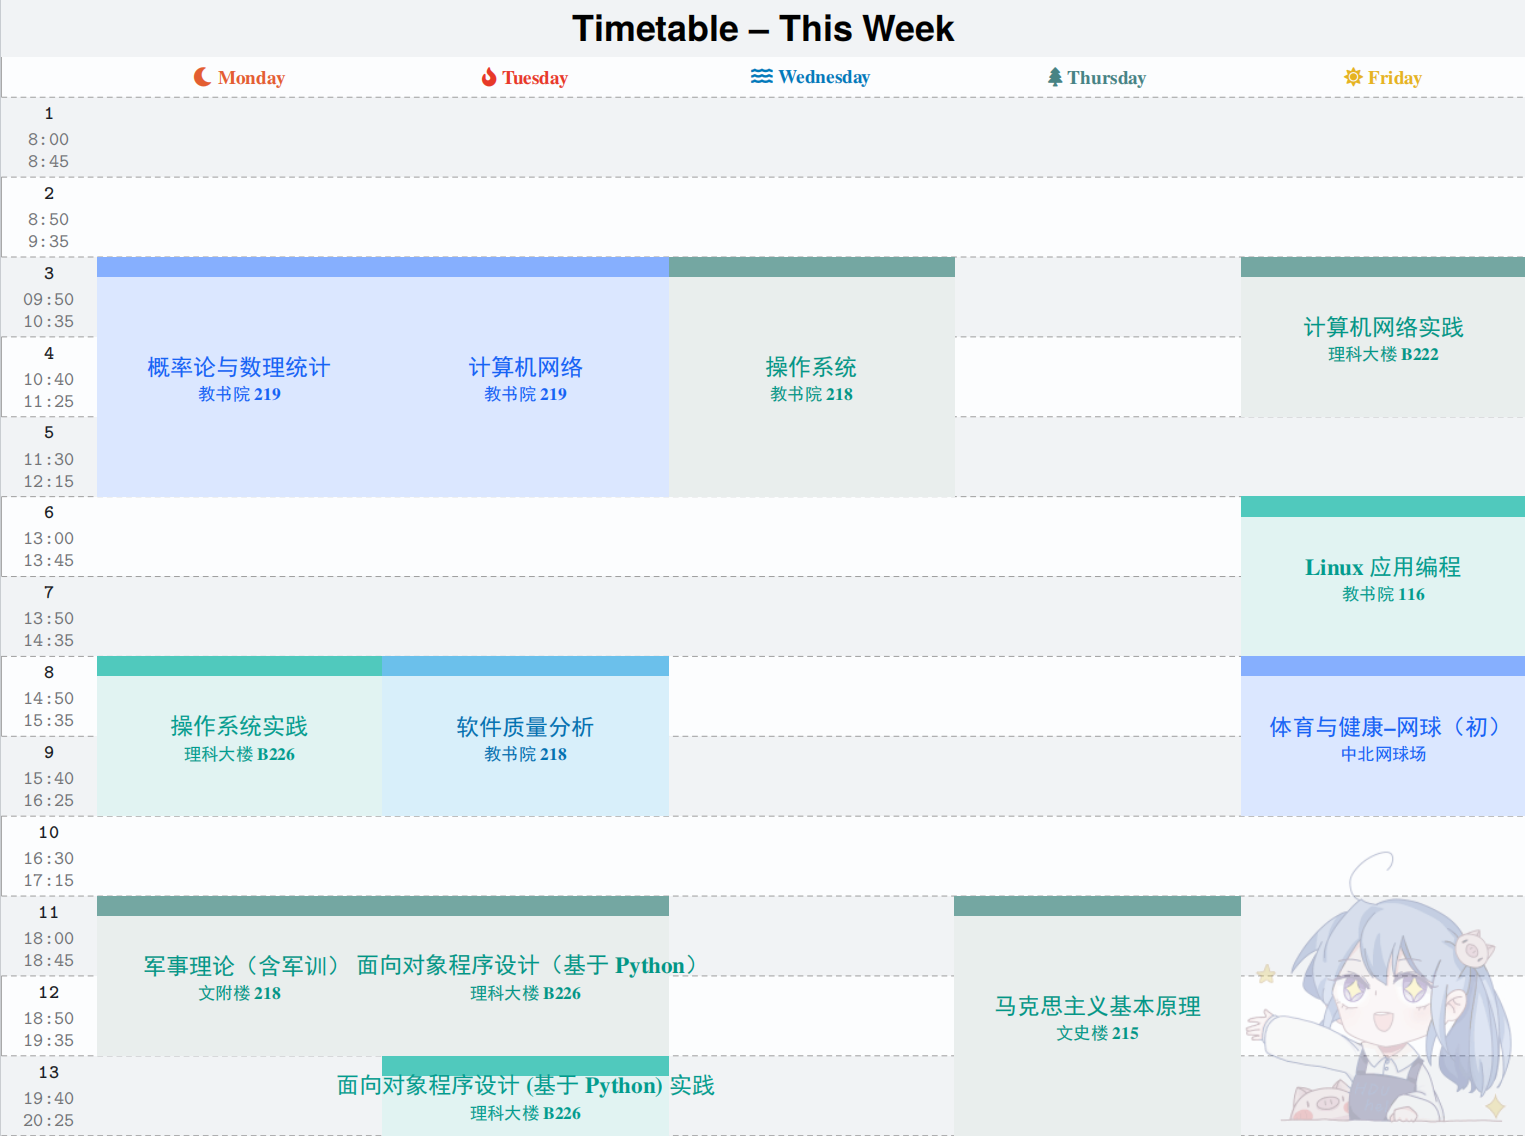
\includegraphics[width=0.6\textwidth]{img/classtable_example.png}
    \caption{LateX 课表生成示例}
    \label{fig:latex_table}
\end{figure}

\subsubsection{文件复制到系统剪贴板}

\begin{note}
    本模块位于 \texttt{src/cpp/copyfile\_build} 中。请查阅相关代码。

    我们使用 \texttt{CF\_HDROP} 数据格式进行 Windows 的文件复制入剪贴板,这一部分可参考 Microsort 写给开发者们的参考文档:
    \href{https://learn.microsoft.com/en-us/windows/win32/shell/clipboard#cf_hdrop}{\underline{https://learn.microsoft.com/en-us/windows/win32/shell/clipboard\#cf\_hdrop}}
\end{note}

\begin{figure}[H]
    \centering
    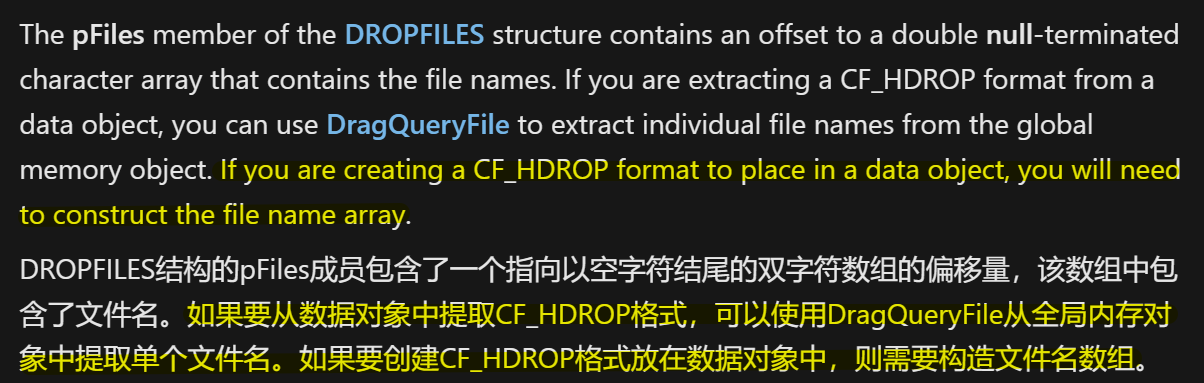
\includegraphics[width=0.578\textwidth]{img/CF_HDROP.png}
    \caption{Microsoft Study Doc - CF\_HDROP}
    \label{fig:copyfile_to_clipboard}
\end{figure}

\textbf{CopyFileToClipboard} 函数是用来将一个文件路径复制到剪贴板的,使用 Windows API 实现。使用 \textbf{CF\_HDROP} 数据格式,它是 Windows 剪贴板的标准格式,用于表示文件路径。具体步骤:

\begin{enumerate}
    \item 调用 \textbf{OpenClipboard} 打开剪贴板,清空剪贴板数据 (\textbf{EmptyClipboard})。
    \item 分配内存 (\textbf{GlobalAlloc}),创建一个 \textbf{DROPFILES} 结构体,其中存储文件路径。
    \item 使用 \textbf{GlobalLock} 锁定分配的内存并填充数据,调用 \textbf{SetClipboardData} 将文件路径放到剪贴板中。
    \item 最后释放内存并关闭剪贴板 (\textbf{CloseClipboard})。
\end{enumerate}

\subsubsection{微信交互接口}

\begin{note}
    微信交互接口是我们最初的设计设想,Python 接管键鼠实现自动化办公,主要使用的是 uiautomation 库,
    它可以实现对 Windows 系统的 UI 自动化操作。

    \vspace{0.3cm}

    在项目中,我们实现了部分和微信有关的接口,能够为后续的开发者们提供逻辑参考。
    在此我们提供一个示例,将生成的 LaTeX 课表通过 CPP 文件复制到微信指定窗口并发送。
\end{note}

\vspace{0.2cm}

\begin{forest}
    for tree={
        grow=east,
        draw,
        edge={-latex},
        rounded corners,
        node options={align=center},
        anchor=west,
        parent anchor=east,
        child anchor=west,
        delay={where content={}{shape=coordinate}{}} % 避免错误节点
    }
    [Root
    [src
    [wechat
    [\_\_init\_\_.py]
    [pc.py]
    [window.py]
    ]
    ]
    [tests
    [test\_wechat
    [test\_pc.py]
    [test\_window.py]
    ]
    ]
    ]
\end{forest}

\begin{itemize}
    \item \textbf{描述}: 封装微信的各种操作,如发送消息、图片、文件等。
    \item \textbf{方法}:
    \begin{enumerate}
        \item \texttt{open\_window()}: 唤起微信窗口并获取窗口控制对象。
        \item \texttt{close\_window()}: 关闭微信主窗口。
        \item \texttt{search(cls, pattern: str)}: 在微信搜索框中输入搜索内容并执行搜索。
        \item \texttt{locate\_chat(cls, name: str | None = None)}: 获取聊天窗口的输入框控件。
        \item \texttt{switch\_to(cls, name: str)}: 切换到指定名称的聊天窗口。
        \item \texttt{send\_message(cls, name: str, text: str)}: 向指定聊天对象发送文本消息。
        \item \texttt{send\_img(cls, name: str, img: str | typing.BinaryIO)}: 向指定聊天对象发送图片。
        \item \texttt{send\_file(cls, name: str, filepath: str)}: 向指定聊天对象发送文件。
    \end{enumerate}
\end{itemize}
